\chapter{预测模型} % Introduction chapter suppressed from the table of contents

有数据才可以做统计分析,下面利用一个案例,芬兰某商业银行的软件维护数据统计分析,简单介绍统计分析的步骤与结果。

先看总体分析结论,再看从原始数据到分析结果的步骤。 
%\hypertarget{ux82acux5170ux67d0ux5546ux4e1aux94f6ux884cux7684ux8f6fux4ef6ux7ef4ux62a4ux6570ux636eux7edfux8ba1ux5206ux6790}{%
%\section{芬兰某商业银行的软件维护数据统计分析}\label{ux82acux5170ux67d0ux5546ux4e1aux94f6ux884cux7684ux8f6fux4ef6ux7ef4ux62a4ux6570ux636eux7edfux8ba1ux5206ux6790}}

%\hypertarget{ux603bux7ed3ux62a5ux544a}{%
%\subsection{芬兰某商业银行的软件维护数据统计分析}\label{ux603bux7ed3ux62a5ux544a}}

%先看总体分析结论,再看从原始数据到分析结果的步骤。

\hypertarget{ux603bux7ed3ux62a5ux544a}{%
\subsection{银行案例总结报告}\label{ux603bux7ed3ux62a5ux544a}}

\hypertarget{ux80ccux666f}{%
\subsubsection{背景}\label{ux80ccux666f}}

银行管理层理解,如果不监控维护工作量,很可能会失控
例如,有些软件系统因为在开发期间没有管理好(例如,引起很多缺陷),就会影响到后面维护工作量提升
所以从86年开始,都一直统计软件维护相关数据。

\begin{itemize}
\tightlist
\item
  从1987年到1995年,银行开发了250
  IBM应用软件,其中部分是系统迁移(从原来的BULL主机迁移到IBM主机)
\item
  從中抽取了67有充分数据的应用软件,做统计分析。
\end{itemize}

希望解答以下问题:

\begin{enumerate}
\tightlist
\item
  那些因素主要影响软件维护工作量(成本)
\item
  有什么办法可以降低维护成本
\item
  利用预测模型,预估下一年度的维护成本
\end{enumerate}

\hypertarget{ux5f71ux54cdux7ef4ux62a4ux5de5ux4f5cux91cfux7684ux4e3bux56e0}{%
\subsubsection{1.影响维护工作量的主因}\label{ux5f71ux54cdux7ef4ux62a4ux5de5ux4f5cux91cfux7684ux4e3bux56e0}}

%\href{文件:maxwell_t5.4.jpg}{文件:maxwell t5.4.jpg}

\includegraphics[width=10cm]{maxwell_t54.jpg}

五个因素代表了62\%的原因:

\begin{itemize}
\tightlist
\item
  第一因素
\end{itemize}

是软件的规模大小占27\% 你可能疑问为什么没有看到缺陷 密度?
因为缺少密度与规模大小,息息相关相关, 所以只需要考虑规模便可以

\begin{itemize}
\tightlist
\item
  第二因素
\end{itemize}

批量处理的集成度

\begin{itemize}
\tightlist
\item
  第三因素
\end{itemize}

是哪一类应用软件,看下图

%\href{文件:maxwell_f5.2.jpg}{文件:maxwell f5.2.jpg}

\includegraphics[width=10cm]{maxwell_f52.jpg}

股票买卖相关的维护工作量最高 一般银行应用,例如捐款转钱最低
原因:股票买卖的规则很复杂,大家都想高竞争力,导致没有标准的模式

\begin{itemize}
\tightlist
\item
  第四因素\\
\end{itemize}

是变更管理的灵活性,如果应用很依赖其他系统更多的利益相关者,需要商户协商达成一致才可以变更,维护成本就低了

\begin{itemize}
\tightlist
\item
  第五因素\\
\end{itemize}

最后一个因素是应用软件投产后多少个月大概每年降低17.4\%,例如,如果第一年是100小时,第二年就会降到82.6小时,下一年会降到68.2小时

\hypertarget{ux4ec0ux4e48ux529eux6cd5ux53efux4ee5ux964dux4f4eux7ef4ux62a4ux6210ux672c}{%
\subsubsection{2.什么办法可以降低维护成本}\label{ux4ec0ux4e48ux529eux6cd5ux53efux4ee5ux964dux4f4eux7ef4ux62a4ux6210ux672c}}

初步分析发现,使用Telon语言的系统要维护工作量较少, 只要1.19小时/FP,
相对不使用Telon的软件系统需要是2.47小时/FP。

针对使用Telon语言的十一个系统统计分析:

\begin{itemize}
\tightlist
\item
  发现语言的百分比与维护工作量正相关;使用的比例越高,维护工作量越低
\item
  用功能点规模归一以后的维护工作量,也是强相关
\end{itemize}

%\href{文件:maxwell_t5.6.jpg}{文件:maxwell t5.6.jpg}

\includegraphics[width=10cm]{maxwell_t56.jpg}

\hypertarget{ux9884ux4f30ux4e0bux4e00ux5e74ux5ea6ux7684ux7ef4ux62a4ux6210ux672c}{%
\subsubsection{3.预估下一年度的维护成本}\label{ux9884ux4f30ux4e0bux4e00ux5e74ux5ea6ux7684ux7ef4ux62a4ux6210ux672c}}

统计分析,除了帮我们洞察那些主要影响因素外,也可以帮我们预测:

%\href{文件:maxwell_t5.5.jpg}{文件:maxwell t5.5.jpg}

\includegraphics[width=10cm]{maxwell_t55.jpg}

但从上表看到模型预测的准确度(Pred(.25)\%)较低,以预测1994年的工作量为例,使用模型预测的准确度还不如直接使用1993年的数据。\\
在前面估算的章节讨论过,有很多因素影响软件开发的工作量,也导致难以准确预估。\\

(注:MMRE = Mean Magnitude of Relative Error, MedMRE = Median MRE ,
Pred(.25)=偏差少于0.25之比例)

\hypertarget{ux6570ux636eux5206ux6790ux6b65ux9aa4}{%
\subsection{银行案例数据分析步骤}\label{ux6570ux636eux5206ux6790ux6b65ux9aa4}}

不用误以为只要有统计分析工具,把项目数据输入,便自动得出上面分析结果。
以下对应每个步骤,用简单例子说明,如想自己动手,使用案例数据,完成整个数据分析过程,请参照Maxwell书里第5章(详见Reference)。

\hypertarget{ux6c47ux603bux6570ux636eux5e76ux660eux786eux6bcfux4e2aux53d8ux91cfux7684ux64cdux4f5cux5b9aux4e49}{%
\subsubsection{汇总数据,并明确每个变量的操作定义}\label{ux6c47ux603bux6570ux636eux5e76ux660eux786eux6bcfux4e2aux53d8ux91cfux7684ux64cdux4f5cux5b9aux4e49}}

\begin{itemize}
\tightlist
\item
  本来数据分散在三个电子表单,每个表单有两百多个项目数据,但很多数据不齐全
\item
  最终汇总出67个项目数据,它们都在1993年有数据
\item
  明确每个变量的操作定义(本来数据表都是用芬兰语言,也有很多银行专业术语),确保大家的理解一致
\end{itemize}

\hypertarget{ux4f7fux7528ux63cfux8ff0ux6027ux7edfux8ba1ux68c0ux67e5ux6570ux636eux5b8cux6574ux6027ux548cux6b63ux786eux6027}{%
\subsubsection{使用描述性统计检查数据完整性和正确性}\label{ux4f7fux7528ux63cfux8ff0ux6027ux7edfux8ba1ux68c0ux67e5ux6570ux636eux5b8cux6574ux6027ux548cux6b63ux786eux6027}}

\begin{itemize}
\tightlist
\item
  用数据总结功能,找出28个变量的均值 / 标准差 / 最大 / 最小:
\item
  发现某些变量最小值是零,不合理。例如: avetrans, disksp, cpu
\item
  有些变量数据不全,为空,请银行经理尽力填上。例如: r1-r10, dbms,tpms
\end{itemize}

%\href{文件:maxwell_e5.1.jpg}{文件:maxwell e5.1.jpg}

\includegraphics[width=10cm]{maxwell_e51.jpg}

\hypertarget{creation-of-new-variablesux5efaux7acbux65b0ux53d8ux91cf}{%
\subsubsection{建立新变量 Creation of New
Variables}\label{creation-of-new-variablesux5efaux7acbux65b0ux53d8ux91cf}}

例:有些项目是在1993年一月份以后才开始维护,
为了要与其他1993年一月份或者以前已开始的项目可以比较,
创建新变量(acorreff),例如,1993年只是维护了10个月,用了30小时,
就要换成36小时{[}=(30/10)*12{]}

\hypertarget{histogramsux7528ux76f4ux65b9ux56feux521dux6b65ux5206ux6790}{%
\subsubsection{用直方图(Histograms)按下表选对应系数初步分析}\label{histogramsux7528ux76f4ux65b9ux56feux521dux6b65ux5206ux6790}}

\begin{itemize}
\tightlist
\item
  画柱状图发现维护工作量(acorreff),规模大小(totfp),都是极度偏左,
\item
  使用自然对数使它变成较近似正态分布(因为变量不是正态分布,会影响回归分析不准确)
\end{itemize}

%\href{文件:maxwell_f5.6.jpg}{文件:maxwell f5.6.jpg}

\includegraphics[width=10cm]{maxwell_f56.jpg}

%\href{文件:maxwell_f5.8.jpg}{文件:maxwell f5.8.jpg}

\includegraphics[width=10cm]{maxwell_f58.jpg}

\hypertarget{scatter-plotux6563ux70b9ux56fe}{%
\subsubsection{散点图(Scatter
plot)}\label{scatter-plotux6563ux70b9ux56fe}}

\begin{itemize}
\tightlist
\item
  从维护工作量 ln(acorreff) 与规模大小 ln(totfp)
  的散点图,看到两者之间有线性关系
\end{itemize}

%\href{文件:maxwell_f529.jpg}{文件:maxwell f5.29.jpg}

\includegraphics[width=10cm]{maxwell_f529.jpg}

\hypertarget{ux9488ux5bf9ux67d0ux4e2aux53d8ux91cfux770bux5404ux79cdux5206ux7ec4ux7684ux6570ux91cfux548cux7ef4ux62a4ux5de5ux4f5cux91cf}{%
\subsubsection{针对某个变量看各种分组的数量和维护工作量}\label{ux9488ux5bf9ux67d0ux4e2aux53d8ux91cfux770bux5404ux79cdux5206ux7ec4ux7684ux6570ux91cfux548cux7ef4ux62a4ux5de5ux4f5cux91cf}}

例如,在内部业务部门(Internal Business Unit)里再细分:

%\href{文件:maxwell_e5.14.jpg}{文件:maxwell e5.14.jpg}

\includegraphics[width=10cm]{maxwell_e514.jpg}

\begin{itemize}
\tightlist
\item
  存款业务(Deposit)的维护工作量最高
\item
  会计管理(Account)的维护工作量最低
\end{itemize}

\hypertarget{ux76f8ux5173correlationux5206ux6790}{%
\subsubsection{相关(Correlation)分析}\label{ux76f8ux5173correlationux5206ux6790}}

两变量的相关从-1 到 1,
关于这系数的意义,可参考附件。因为如果两个变量是强相关,
如果把这两个高度相关的变量放在一起做预测模型,就会会导致模型不稳定,所以要预先删除、处理。下表是相关系数大于0.51
的汇总表:

例如,因为r2和r3强相关,它们也与其他变量相关,所以决定把r2剔除

\hypertarget{ux56deux5f52ux5206ux6790}{%
\subsubsection{回归分析}\label{ux56deux5f52ux5206ux6790}}

\begin{itemize}
\tightlist
\item
  利用以下连续变量做回归分析 {[}Y是维护工作量(lacorreff){]}
\end{itemize}

\begin{description}
\item[]
\begin{description}
\tightlist
\item[]
(ltotfp, pcobol, pjcl, ageend, ladefect)
\end{description}

ln(acorreff) = 2.532 + 0.541*(ltotfp)

\begin{description}
\tightlist
\item[]
Adj. R-square = 0.27
\end{description}
\end{description}

\begin{itemize}
\tightlist
\item
  最终得出以下5变量回归模型
\end{itemize}

\begin{description}
\tightlist
\item[]
ln(acorreff) = 3.768 + 0.555*ln(totfp) + r9\_coef + submorg\_coef +
r3\_coef - 0.016*ageend

\begin{description}
\tightlist
\item[]
Adj. R-square = 0.619
\end{description}
\end{description}

\begin{itemize}
\tightlist
\item
  r10 因与submorg强相关,被剔除,剩下5变量
\item
  r9, submorg, r3 因为是分组数据,系数会依据类型,按下表选对应系数:
\end{itemize}

%\href{文件:maxwell_e5.14.jpg}{文件:maxwell e5.14.jpg}

%\includegraphics[width=10cm]{maxwell_e514.jpg}

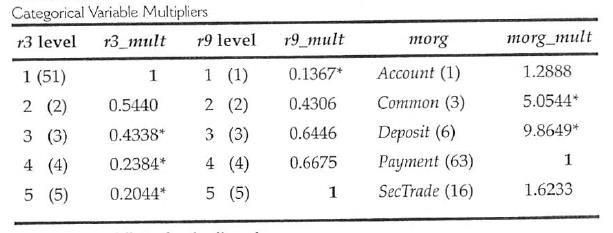
\includegraphics[width=10cm]{Maxwell_t514.jpg}


\hypertarget{ux7528ux56deux5f52ux6a21ux578bux9884ux6d4b}{%
\subsubsection{用回归模型预测}\label{ux7528ux56deux5f52ux6a21ux578bux9884ux6d4b}}

尝试用五个变量的回归方程来预测1994年项目维护工作量:\\
1994年有17个项目,是1993年的延续,直接沿用93年的历史数据来估计94年的工作量(详见下表),发现有35\%可以预测偏差低于25\%。(Pred(.25)
= 35.3\% , MMRE=75.6, MedMRE=41.9)

%\href{文件:maxwell_t5.15.jpg}{550px}

\includegraphics[width=10cm]{maxwell_t515.jpg}

同样,如果用模型来预测这17个项目的工作量,它能预测在25\%之内的百分比更低,只有29.4\%。(Pred(.25)=29.4\%,
MMRE=101.4, MedMRE=56.0)
但是如果是用五个变量的模型来预估94年2个新项目,它在25\%的准确度之内的有50\%。(Pred(.25)=50\%,
MMRE=47.6, MedMRE=47.6)

比较之下,发现这个预测模型用来预估工作量的能力不理想,因为它还不如直接用往年(1993)的数据来估,但可用于估算一些没有历史数据的新项目。

\hypertarget{ux5206ux6790ux4f7fux7528telonux5bf9ux7ef4ux62a4ux5de5ux4f5cux91cfux7684ux4f5cux7528}{%
\subsubsection{分析使用Telon对维护工作量的作用}\label{ux5206ux6790ux4f7fux7528telonux5bf9ux7ef4ux62a4ux5de5ux4f5cux91cfux7684ux4f5cux7528}}

针对11个使用Telon语言的应用软件,计算每一个的维护工作量除以规模大小,得出新变量(mdrate),明显看到这11个比其它56个没有用Telon的应用软件,用Telon的MDRATE明显低(每个功能点只需要1.19个小时),其它是2.47。(详见下表)

%\href{文件:maxwell_e5.31.jpg}{550px}

\includegraphics[width=10cm]{maxwell_e531.jpg}

再针对11个Telon应用软件,发现Telon使用\%与维护工作量有显著的线性关系(看下面的散点图),也可以得出一个回归方程。

%\href{文件:maxwell_f5.53.jpg}{550px}

\includegraphics[width=10cm]{maxwell_f553.jpg}

如果用MDRATE来比较,也可以得出有线性关系的散点图和回归方程,表示不仅仅是Telon占比越多工作量越小,并可以利用回归方程预估维护工作量。

%\href{文件:maxwell_f5.54.jpg}{550px}

\includegraphics[width=10cm]{maxwell_f554.jpg}

\href{文件:maxwell_e5.34.jpg}{550px}

\includegraphics[width=10cm]{maxwell_e534.jpg}

%\hypertarget{ux56deux987eux4e0eux603bux7ed3}{%
%\section{回顾与总结}\label{ux56deux987eux4e0eux603bux7ed3}}

\hypertarget{ux603bux7ed3ux62a5ux544a}{%
\subsection{回顾与总结}\label{ux603bux7ed3ux62a5ux544a}}

统计分析可以帮我们了解:

%Screenshotfrom2023-01-0420-18-25.png

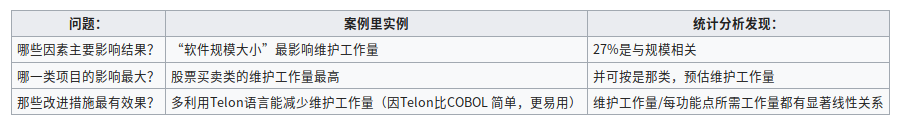
\includegraphics[width=10cm]{Screenshotfrom2023-01-0420-18-25.png}

也可以用作预测, 例如, 预估来年(1994年)项目维护工作量。

但统计分析并非简单按个键就会有分析结果,之前先要做好一系列准备工作,例如:

%Screenshotfrom2023-01-0420-19-06.png

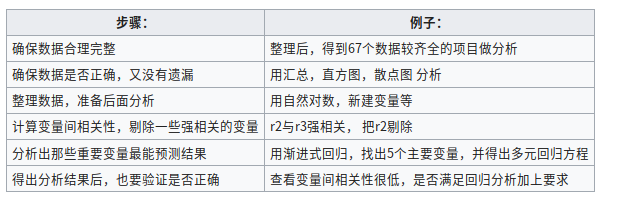
\includegraphics[width=10cm]{Screenshotfrom2023-01-0420-19-06.png}

虽然银行在八年时间内收集了两百多个项目的数据,
但最终只有67个项目数据可用。 所以当初的度量计划很重要,
除了识别那些软件维护相关的数据需要收集外,
也要预先想好度量项的操作定义(以免各有不同理解),如何收集数据,怎样存储,
后面如何分析等。 才能减少收集没有用的数据, 或数据不齐全,影响分析。

也了解到最终预测模型的变量应该不会太多(银行案例:从本来28,最终5个)。
所以无论是机器学习,或基本统计分析目的都是希望可以找出最有用的几个变量,wrapper是其中一种常用的方法,有兴趣多了解,详见附件。

\hypertarget{ux9644ux4ef6}{%
\section{附件}\label{ux9644ux4ef6}}

\hypertarget{ux6848ux4f8bux90e8ux5206ux53d8ux91cfux5217ux8868}{%
\subsection{案例部分变量列表}\label{ux6848ux4f8bux90e8ux5206ux53d8ux91cfux5217ux8868}}

\hypertarget{ux6848ux4f8bux90e8ux5206ux53d8ux91cfux8be6ux79f0ux4e0eux5b9aux4e49}{%
\subsubsection{案例部分变量列表}\label{ux6848ux4f8bux90e8ux5206ux53d8ux91cfux8be6ux79f0ux4e0eux5b9aux4e49}}

%Screenshotfrom2023-01-0420-19-59.png

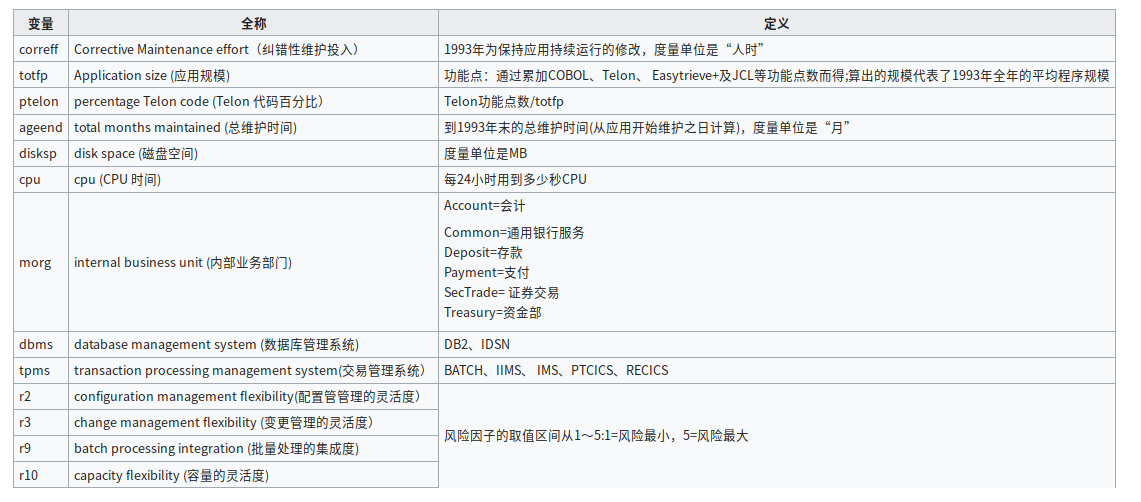
\includegraphics[width=10cm]{Screenshotfrom2023-01-0420-19-59.png}

\hypertarget{ux8fd9ux4e9bux53d8ux91cfux7684ux5f52ux7c7b}{%
\subsubsection{变量的归类}\label{ux8fd9ux4e9bux53d8ux91cfux7684ux5f52ux7c7b}}

%Screenshotfrom2023-01-0420-20-52.png

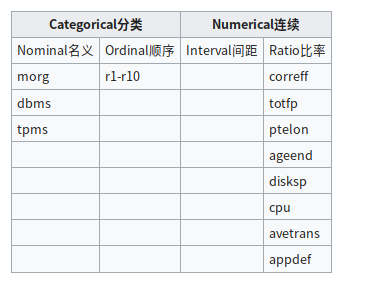
\includegraphics[width=10cm]{Screenshotfrom2023-01-0420-20-52.png}

\hypertarget{ux6309ux53d8ux91cfux5f52ux7c7bux5e38ux7528ux5206ux6790ux5de5ux5177}{%
\subsubsection{按变量归类,常用分析工具}\label{ux6309ux53d8ux91cfux5f52ux7c7bux5e38ux7528ux5206ux6790ux5de5ux5177}}

%\href{文件:maxwell_t6.8.jpg}{文件:maxwell t6.8.jpg}

\includegraphics[width=10cm]{maxwell_t68.jpg}

\hypertarget{x-ux4e0e-y-ux76f8ux5173ux6027ux56fe}{%
\subsection{X 与 Y 相关性图}\label{x-ux4e0e-y-ux76f8ux5173ux6027ux56fe}}

\begin{itemize}
\tightlist
\item
  完美负相关(-1):
\end{itemize}

%\href{文件:maxwell_f6.7.jpg}{文件:maxwell f6.7.jpg}

\includegraphics[width=10cm]{maxwell_f67.jpg}

\begin{itemize}
\tightlist
\item
  零相关(0):
\end{itemize}

%\href{文件:maxwell_f6.9.jpg}{文件:maxwell f6.9.jpg}

\includegraphics[width=10cm]{maxwell_f69.jpg}

\begin{itemize}
\tightlist
\item
  完美正相关(+1):
\end{itemize}

%\href{文件:maxwell_f6.8.jpg}{文件:maxwell f6.8.jpg}

\includegraphics[width=10cm]{maxwell_f68.jpg}

\hypertarget{ux5229ux7528-wrapper-ux964dux4f4eux6a21ux578bux7684ux53d8ux91cf}{%
\subsection{利用 Wrapper
降低模型的变量}\label{ux5229ux7528-wrapper-ux964dux4f4eux6a21ux578bux7684ux53d8ux91cf}}

当我们收集到一定数量的项目数据,就可以尝试做数据分析。很多分析数据时,没有考虑项目之间的差异,假定项目的特性都类似,然后直接就用统计分析方法,求模型的方程式参数。\\

\hypertarget{row-pruning}{%
\subsubsection{Row pruning}\label{row-pruning}}

例如下图是某公司4个项目的6个迭代系统测试缺陷密度数据,你觉得把4个项目的缺陷密度放在一起分析合适吗?很明显两个项目缺陷比较低,有些很散,所以如果没有考虑项目之间的差异,直接总体分析就会变成很宽,做出来的模型预测准确度不会好。

%\href{文件:M4BrowPruningGraphScreenshot_2023-01-04_203004.jpg}{550px}

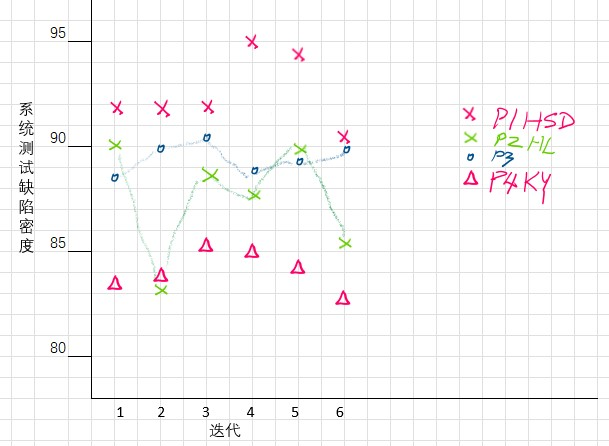
\includegraphics[width=10cm]{M4BrowPruningGraphScreenshot_2023-01-04_203004.jpg}

\hypertarget{column-pruning}{%
\subsubsection{Column pruning}\label{column-pruning}}

除了要细分项目就是要考虑保留那些项目参数(影响因素),很多时候我们看到一些公司级的数据分析,一个大堆表可能有三十多个变量,从模型出来的变量越多,其实不是好事:

\begin{enumerate}
\tightlist
\item
  可能做了过度的调整,导致那个预测模型没有预测的意义,只适合用在这堆项目数据上;
\item
  变量多也会导致要花很多精力去收集数据,不划算。
\item
  使用模型的人也很难理解这个模型的意义,不知道如何去使用。\\
\end{enumerate}

我们在前面EST2里的乐高模型数据案例,简单用了两个变量来做个预测模型:

\begin{enumerate}
\tightlist
\item
  积木的数量,即它的规模大小;
\item
  团队人数;可以比较好地估计工作量,这是比较理想的模型。\\
\end{enumerate}

所以当开始时,收集到很多变量,我们就需要利用数据分析删除一些意义不大的变量。\\
怎么挑选呢?\\
比如一个方式是用wrapper机械性地去挑选,如果增加一个变量准确度更好就增加,如果不是就不增加,直到挑选出最佳的搭配。

数据裁剪(pruning)后不会因为减少了数据而影响预测的准确度,例如看左图,红线是本来的4组数据的预测准确度\%,绿色是做了裁剪后的准确度,虽然有提升但不多,原因是只是做了column
pruning
,裁剪栋(变量),没有其它。右图是对8个NASA的项目做数据裁剪,利用wrapper工具,除了做column
pruning外,也做大量row
pruning,减少数据的列,结果:除了c03外,其它7个项目的预测准确度都有明显提升。中间图是针对call、pall、tall三组数据,call是C01,C02加C03同样的,pall包括p02,
p03和p04,tall包括t02和t03,因为每组都是由几个数据包合成,所以可减少的列有限,准确度的提升也没有右图那么大。

%\href{文件:chen_f3.jpg}{600px}

\includegraphics[width=10cm]{chen_f3.jpg}

从对这些公开数据的小实验看到,利用数据裁剪不会因为减少了列和栋,影响预测的准确度,反而会提升,而且如果不仅裁剪栋(column
pruning),同时也裁剪列(row pruning),预测的准确度提升可能越多。

\framebox{%
\begin{minipage}[t]{0.97\columnwidth}\raggedright
数据包说明:

cii0是COCOMO-II模型的数据包

cii4包括cii0的7个项目,加上47个1990年后新项目

coci数据包括各种工程、科学、财务等领域项目

na60数据包包括美国NASA 20年的项目数据,里面包括:

\begin{itemize}
\tightlist
\item
  c01、c02、c03,从三个不同NASA地域收集的数据
\item
  p02、p03、p04 数据来自三个NASA项目
\item
  t02、t03 数据来自包括地面数据收集(ground-data receiving)和导航(flight
  guidance)两类NASA项目
\end{itemize}

call、pall、tall三组数据:

\begin{enumerate}
\tightlist
\item
  call是C01,C02和C03
\item
  pall包括p02, p03和p04
\item
  tall包括t02和t03
\end{enumerate}\strut
\end{minipage}}

\hypertarget{ux5982ux4f55ux505aux56deux5f52ux5206ux6790}{%
\subsection{如何做回归分析}\label{ux5982ux4f55ux505aux56deux5f52ux5206ux6790}}


1.确定哪些关系将被研究。\\

2.收集x和y变量的数据。\\

3.通过在x轴绘制独立变量和在y轴绘制因变量,设立一条拟合线图。\\

4.创建拟合线\\


\begin{itemize}
\tightlist
\item
  如果手动创建拟合线图,穿过那些值画一条直线,这条直线在线与单独的标出点(最适合)之间保留总空间的最少量。
\item
  如果使用电脑程序,通过``最小二乘法''计算并绘制这条线。
\end{itemize}

%\url{文件:相关性09.png}

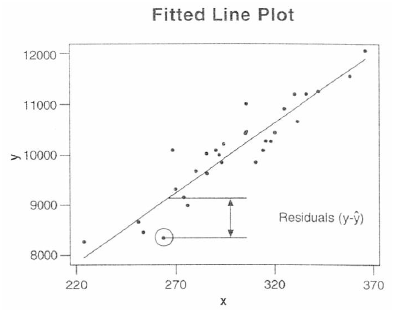
\includegraphics[width=10cm]{相关性09.png}\\

5.计算相关系数r (x和y之间的相关性,从 -1 到 +1)\\

6.通过使用方程式y=mx+b,确定斜率或线的y轴截距。\\


\begin{itemize}
\tightlist
\item
  y截距是``最佳拟合线''穿过的在y轴上的点(在这一点,x=0)。
\item
  线的斜率(m)按照y的变化除以x的变化来计算(m=∆y/∆x)。斜率m也认作预测变量x的系数。
\end{itemize}


7.计算残差(residuals)\\


\begin{itemize}
\tightlist
\item
  在对于任何给定的x的预测反应变量(叫做
  \(\hat y\))和实验值或者实际响应(y)之间的区别叫做残差(e=y -
  \(\hat y\))。残差用来确定模型是否好使用。残差的估算标准差是关于回归线的错误项的度量
\end{itemize}


8.确定重要性 (significance),执行t-检验(在计算机的帮助下)并为每个因素计算p-值。\\


\begin{itemize}
\tightlist
\item
  少于α (通常是0.05)的p-值将指示一个统计上的重要关系。
\end{itemize}

9.使用方差分析法(ANOVA)分析整个模型是否具备显著关系,分析报告包括F-检验结果与相关p-值

10.计算R\textsuperscript{2}和R\_adj\textsuperscript{2}。


\begin{itemize}
\tightlist
\item
  R\textsuperscript{2},判定系数,是相关系数的平方并且度量由模型解释的变量的比例。理想上,R\textsuperscript{2}应该等于1,表示零误差。
\end{itemize}

%\url{文件:相关性10.png}

%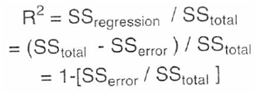
\includegraphics[width=10cm]{相关性10.png}

\[{R}^2 = {SS}_{regression} / {SS}_{total}\]\\
\[= ( {SS}_{total} - {SS}_{error} ) / {SS}_{total}\]\\
\[= 1 - [ {SS}_{error} / {SS}_{total} ]\]\\

其中SS=平方和

\begin{itemize}
\tightlist
\item
  R\_adj\textsuperscript{2}是考虑了模型中项数和数据点的数量的R\textsuperscript{2}的修正测量。
\end{itemize}

%\url{文件:相关性11.png}

%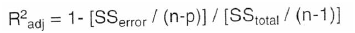
\includegraphics[width=10cm]{相关性11.png}

\[{R}_{adj}^2 = 1 - [{SS}_{error} / (n - p)] / [{SS}_{total} / (n - 1)]\]

其中n=数据点的数量并且p=模型中的项数。模型中的项数也包括常数。

注意:不像R\textsuperscript{2},当增加提供很少新信息的条款并且随着模型条款的数量越靠近总样本大小时,R\_adj\textsuperscript{2}可能变得更小,。理想上,R\_adj\textsuperscript{2}应该是最大化,尽可能靠近R\textsuperscript{2}。

结论应该被验证,尤其当历史数据已经被使用时。

使用历史数据验证回归模型。

%例子:想确定在为每一个特定产品分配的货架空间的数量和对同样的产品的销售量之间是否存在关系。她调查同样链的30个不同的商店,所有的都有相似的人口统计资料。比较分配的货架空间(x)和销售(y)收集数据。使用一个计算机程序来运行方差分析显示了下面的结果:

\hypertarget{ux80ccux666f}{%
\subsubsection{例子}\label{ux80ccux666f}}

想确定在为每一个特定产品分配的货架空间的数量和对同样的产品的销售量之间是否存在关系。调查同样链的30个不同的商店,所有的都有相似的人口统计资料。比较分配的货架空间(x)和销售(y)收集数据。使用一个计算机程序来运行方差分析显示了下面的结果:

%\url{文件:相关性12.png}

%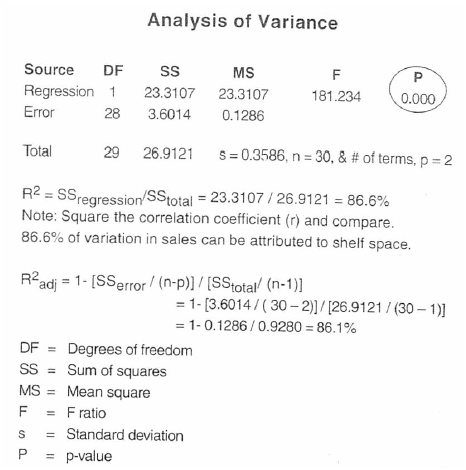
\includegraphics[width=10cm]{相关性12.png}

%\href{文件:Ch24rrScreenshot_2023-04-02_094408.jpg}{450px}

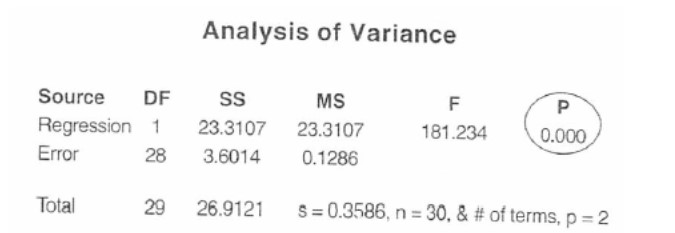
\includegraphics[width=10cm]{Ch24rrScreenshot2023-04-02094408.jpg}

\[{R}^2 = {SS}_{regression} / {SS}_{total} = 23.3107 / 26.9121 = 0.866\]\\
注: 销售变化的 0.866与 货架空间有关\\

\[{R}_{adj}^2 = 1 - [{SS}_{error} / (n - p)] / [{SS}_{total} / (n - 1)]\]\\
\[= 1 - [3.6014 / (30 - 2)] / [26.9121 / (30 - 1)]\]\\
\[= 1 - 0.1286 / 0.928 = 0.861\]\\

\begin{description}
\tightlist
\item[]
DF = Degrees of freedom (自由度)\\
SS = Sum of squares (平方和)\\
MS = Mean Square (均方)\\
s = Standard deviation (标准差)\\
P = p-value ( P值)\\
\end{description}

相关性分析显示一个强的正相关(r=+0.931)。

%\url{文件:相关性13.png}

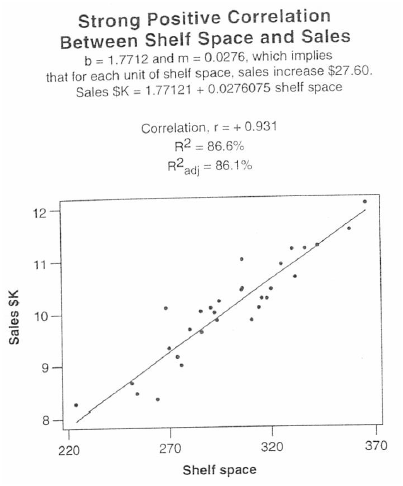
\includegraphics[width=10cm]{相关性13.png}

用以下4图分析残差以验证回归/方差分析是否满足回归分析的假设条件:\\
%\url{文件:相关性15.png}~\\

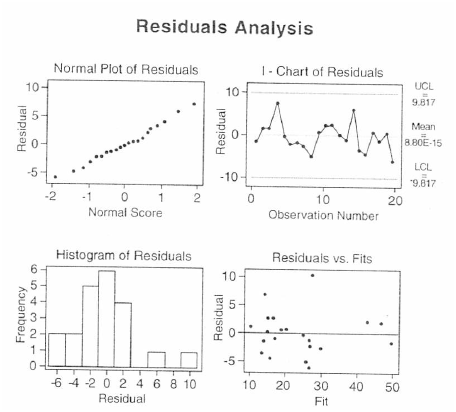
\includegraphics[width=10cm]{相关性15.png}
例:右面两残差图看残差是否平均上下分散?左面两图看是否正态分布?

\hypertarget{references}{%
\section{References}\label{references}}

1. Maxwell, Katrina: \emph{Applied Statistics for Software Managers}
Prentice-Hall 2002.\\
2. Chen, Zhihao: "Finding the Right Data for Software Cost Modeling"
IEEE Software Nov/Dec 2005\\
3. Six Sigma Academy:''The Black Belt Memory Jogger'' GOAL/QPC 2002.\\




